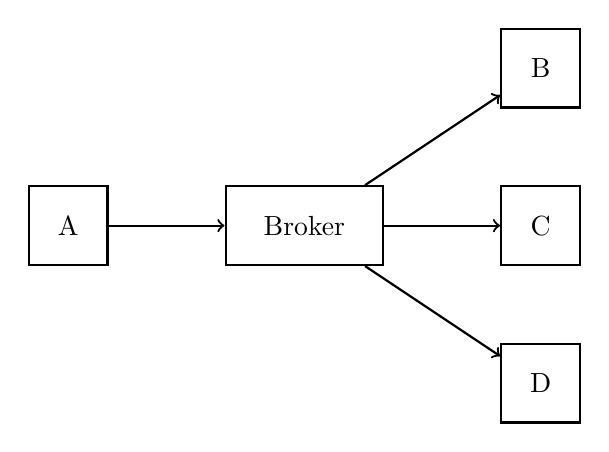
\begin{tikzpicture}[thick]
  \node(A) [draw,rectangle,minimum width=1cm,minimum height=1cm]{A};

  \begin{scope}[xshift=3cm]
    \node(Broker) [draw,rectangle,minimum width=2cm,minimum height=1cm]{Broker};
  \end{scope}

  \begin{scope}[xshift=6cm, yshift=2cm]
    \node(B) [draw,rectangle,minimum width=1cm,minimum height=1cm]{B};
  \end{scope}

  \begin{scope}[xshift=6cm]
    \node(C) [draw,rectangle,minimum width=1cm,minimum height=1cm]{C};
  \end{scope}

  \begin{scope}[xshift=6cm, yshift=-2cm]
    \node(D) [draw,rectangle,minimum width=1cm,minimum height=1cm]{D};
  \end{scope}

  \draw[->] (A) edge (Broker)
            (Broker) edge (B)
            (Broker) edge (C)
            (Broker) edge (D);
\end{tikzpicture}
